\chapter[Estratégias evolutivas para o PRM]{Estratégias evolutivas para o PRM}

A modelagem de um algoritmo genético para o problema do roteamento multicast não é trivial, pois a solução não pode ser representada por um vetor. De fato, como deve representar os caminho entre o servidor e os múltiplos destinos em uma rede de computadores, a solução para o PRM é melhor representada por uma árvore. Dessa forma, é preciso desenvolver o processo de crossover e de mutação de acordo com essa estrutura. O operador de cruzamento deve receber duas árvores pais e gerar uma nova árvore (filha) que compartilha características de ambos os pais. O operador de mutação precisa criar uma pequena alteração na árvore que permita explorar diferentes regiões do espaço de busca, mas que não a descaracterize completamente.

Em contrapartida, o PRM se aproxima da definição original do ACO, pois trabalha com grafos. A diferença está no fato de que a solução é representada por uma árvore ao invés de um simples caminho, fazendo com que o depósito de feromônio e a escolha de arestas sejam desenvolvidas conforme a nova estrutura.

\section{Representação da solução}

Como mostrado na seção \ref{section_problemas_prm}, considerando que em cada nó da rede a mensagem pode ser replicada e enviada aos próximos nós conectados, o PRM deseja encontrar a árvore que representa o processo de transmissão de menor custo que parte do nó fonte (servidor) e atinge todos os destinos. Existem duas maneiras de se representar uma solução:

\begin{enumerate}
	\item \textbf{Representação em árvore:} \cite{Bueno2010} o AG evolui a própria árvore que se deseja encontrar como solução. É um processo mais complicado que elimina a necessidade de pós-processamento. A \autoref{fig_prm_mono}, na seção \ref{section_problemas_prm}, mostra alguns exemplos de árvores multicasts.
	\item \textbf{Representação em conjunto:} \cite{Baran2004} o AG evolui um conjunto de caminhos $C$, ou seja, para cada nó destino $d$, deve existir uma sequência de nós $L \in C$ que contém o caminho que leva do nó servidor (emissor) até o nó $d$. A representação em conjuntos de caminhos é mais fácil de se gerenciar, mas exige a transformação (conjunção) dos caminhos pertencentes ao conjunto em uma árvore  ao final do processo. Como diferentes árvores podem ser formadas a partir de um único conjunto de caminhos, essa representação não é tão eficiente quanto a anterior ao explorar o espaço de busca.
\end{enumerate}

Neste trabalho, optou-se por utilizar a representação em árvores.

\section{Inicialização dos indivíduos}
Considere um grafo da rede $G$, um nó raiz (também chamado de servidor ou emissor) $r$ e um conjunto de nós de destino $D$, para criar uma solução aleatória no PRM, inicia-se um grafo $S$ apenas com o vértice $r$, o passo seguinte é extrair um destino aleatório $d \in D$ e, com base no grafo $G$, criar um caminho em $S$ entre qualquer um de seus vértices atuais e $d$. Após construir o caminho, $d$ com certeza será atingível a partir de qualquer vértice de $S$. O processo se repete até que todos os nós destinos estejam no grafo $S$. Por fim, o grafo $S$ é transformado em uma árvore a partir da remoção dos ciclos presentes em $S$ e da aplicação de podas dos ramos desnecessários.

Para criar o caminho aleatório entre um vértice de $S$ e um nó destino $d$, considera-se um vetor de exploração $Exp$ que, inicialmente, contém todos os nós de $S$. Enquanto o destino $d$ não é encontrado, algum nó $exp_i \in Exp$ é escolhido e todos os vértices adjacentes (conectados) a $exp_i$ são incluídos em $Exp$. Quando $d$ é encontrado, adiciona-se a $S$ o caminho necessário para sair de algum vértice de $S$ e chegar ao destino $d$.

\section{Cruzamento (AG)}

A estratégia de cruzamento utilizada neste trabalho para o PRM é chamada de cruzamento por caminho e foi proposta em \cite{Lafeta2016} como alternativa ao cruzamento por similaridade utilizado em trabalhos anteriores \cite{Bueno2010}. Esse tipo de cruzamento é realizado entre duas árvores $P_1$ e $P_2$ e produz um único filho $F$. O processo consiste em separar cada um dos pais em ramos e, então, para cada nó destino $d$, acrescentar a $F$ o ramo de $P_1$ ou de $P_2$ que leva a $d$. A escolha entre $P_1$ e $P_2$ é feita de forma aleatória. Assim que todos os nós destinos são atingíveis em $F$, a etapa de seleção de ramos é interrompida, os ciclos que possivelmente foram criados são removidos, e um processo de poda é realizado a fim de remover qualquer nó folha que não seja destino.

\begin{figure}[!htbp]
	\label{fig_prm-cruzamento-caminho}
	\centering
	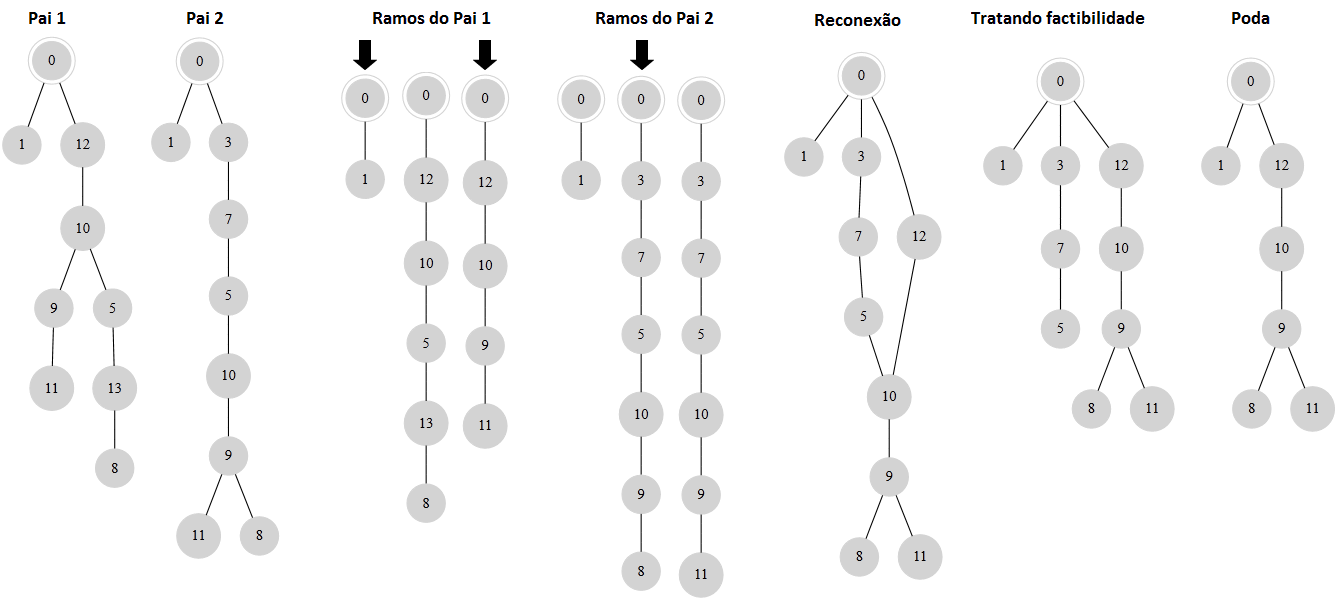
\includegraphics[width=1\textwidth]{cap_estrategias-prm/figs/prm-cruzamento-caminho}
	\caption{Exemplo de cruzamento por caminho. Retirado de \cite{LafetaThesis}}
\end{figure}

A figura \ref{fig_prm-cruzamento-caminho}, retirada do trabalho de \cite{Lafeta2016}, representa o processo de cruzamento por caminho entre duas árvores (Pai 1 e Pai 2). No exemplo, o nó raiz é o vértice 0 e os nós destinos são o conjunto $\{1, 8, 11\}$. As setas em ``ramos do pai 1'' e ``ramos do pai 2'' representam os caminhos escolhidos em cada um dos pais para compor a árvore filha. O grafo nomeado ``reconexão'' representa o filho após a inclusão de todos os ramos. Como foi gerado um ciclo, o mesmo deve ser removido a fim de obter uma árvore válida. Em ``tratando factibilidade'', apresenta-se o filho após a remoção dos ciclos. Como o nó folha 5 não é um destino, ele é removido durante o processo de poda, resultando na última árvore (``poda'') que é o filho resultante do processo.

Para remover os ciclos, percorre-se a árvore em largura removendo qualquer aresta que adicione ciclo. No processo de poda, verifica-se todas as folhas. Se algum nó folha não for um destino, ele é removido e o processo repetido até que todos os nós folhas sejam destinos.

Após o cruzamento, realiza-se um processo de filtragem, onde todas as soluções repetidas são substituídas por novos indivíduos gerados aleatoriamente.

\section{Mutação (AG)}

A mutação em uma árvore que representa uma solução para o PRM consiste em remover parte dos nós da árvore e então reconectá-los de maneira aleatória utilizando o grafo correspondente à rede em questão. As etapas desse processo estão descritas no o algoritmo \ref{alg_prm_mutacao}.

\begin{algorithm}
	\caption{Mutação para uma árvore $(A, G, qte_{arestas}, r, D)$}
	\label{alg_prm_mutacao}
	\begin{algorithmic}[1]
		\State desconectar($A$, $qte_{arestas}$)
		\State $C \gets extraiComponente(A, r)$
		\State $M \gets novoGrafo()$
		\State $M \gets mesclar(M, C)$
		\While{$|D| > 0$}
		\State $d \gets removeAleatorio(D)$
		\State $C \gets extraiComponente(A, d)$
		\If{$d \notin V(M)$}
		\State $P \gets caminhoAlearorio(C, M, G)$
		\State $M \gets mesclar(M, P)$
		\EndIf
		\State $M \gets mesclar(M, C)$
		\EndWhile
		\State $removerCiclos(M)$
		\State $podarArvore(M)$
		\State \Return $M$
	\end{algorithmic}
\end{algorithm}

O algoritmo recebe como entrada a árvore que sofrerá mutação ($A$), o grafo da rede ($G$), a quantidade de arestas a se remover na mutação ($qte_{arestas}$), o vértice raiz ($r$), e o conjunto de destinos ($D$). Na linha 1, desconecta-se a árvore através da remoção aleatória de $qte_{arestas}$ arestas. Entre as linhas 2 e 4, cria-se a estrutura para a construção da árvore. A partir da linha 5 começa o laço para reconectar todos os nós destinos à arvore. A linha 6 seleciona um destino aleatório $d$ para reconectar. Na linha 7, a componente conexa contendo $d$ é extraída de $A$ e chamada de $C$. Se não existe componente conexa com o vértice $d$, $C$ será um grafo com um único nó ($d$) e nenhuma aresta. Caso o vértice $d$ não exista na componente conexa $M$, cria-se um caminho aleatório em $M$ (com base no grafo $G$) que a conecta a $C$ (linhas 8 a 10). A construção do caminho aleatório é feita nó a nó até se encontrar uma sequência de arestas entre as duas componentes. Na linha 11, inclui-se em $M$ todas as arestas de $C$. Ao final, o mesmo pós-processamento do cruzamento por caminho é realizado: remoção de ciclos e poda da árvore (linhas 14 e 15).

\section{Construção da solução (ACO)}
\label{section_estrategias_prm_aco}

O processo de construção da solução por um ACO no PRM deve gerar a árvore \textit{multicast} com base no grafo da rede, da estrutura de feromônios e da heurística. Existem diversas maneiras de se criar tal árvore. A fim de estudar o comportamento das diferentes estratégias possíveis, aprimorá-las e determinar o melhor modelo para se utilizar no PRM, analisou-se o comportamento de cada ideia no caso mais básico possível: o PRM mono-objetivo. As ideias consideradas neste trabalho são listadas a seguir:

\begin{enumerate}
	\item A primeira estratégia, apresentada em \cite{Pinto2005}, pode ser vista como uma formiga que caminha pelo grafo até encontrar todos os destinos. A análise é feita passo a passo, considerando apenas a vizinhança do vértice corrente como possibilidades para compor a solução. O processo inicia com uma lista de exploração ($Exp$) que contém um único elemento: a raiz. Sorteia-se um vértice $i \in Exp$ e atribui-se probabilidades a todas as arestas $(i, j)$, onde $j$ é qualquer vértice não-visitado na adjacência de $i$. $i$ é removido de $Exp$ caso não possua vizinhos factíveis. Um vértice $v$ é escolhido de acordo com as probabilidades calculadas (conforme à seção \ref{section_otimizacao_aco_construcao}), a aresta $(i, v)$ é adicionada à solução e $v$ é inserido na lista de exploração $Exp$. O processo é repetido até que todos os destinos tenham sido alcançados. Como etapa final, poda-se a árvore, eliminando as folhas que não representam destinos.
	\item Uma solução pode ser vista como os caminhos entre a raiz e cada um dos destinos. Portanto, outra estratégia é imaginar que $|D|$ formigas partirão da raiz e cada uma deve encontrar um vértice $d \in D$ diferente, sendo $D$ o conjunto de nós destinos. Com os caminhos para todos os nós destinos definidos, monta-se a árvore evitando a ocorrência de ciclos. Por fim, realiza-se a poda da árvore para excluir qualquer vértice folha que não seja um destino. %mants
	\item Uma terceira estratégia é proposta neste trabalho. Ela adota uma representação de formiga fictícia que pode estar em vários locais do grafo ao mesmo tempo (formiga com sobreposição quântica). Dessa forma, é possível analisar as probabilidades de todas as arestas factíveis ao mesmo tempo, ao invés de sempre escolher a composição da solução de acordo com uma vizinhança local. Ao considerar todas as possibilidades ao mesmo tempo, obtém-se um processo melhor de decisão que não apresenta qualquer tendência (viés) para algum dos ramos da árvore, já que a todo momento, qualquer vértice factível pode ser incluído no resultado. O processo é iniciado a partir de uma lista de exploração ($Exp$) que contém todas as arestas conectadas ao nó raiz. A cada passo, calcula-se as probabilidades para toda aresta de $Exp$ e, de acordo com os valores obtidos, escolhe-se $exp_i \in Exp$ para compor a solução. $exp_i$ é então removida de $Exp$, adicionada à solução e tem todas suas arestas adicionadas à lista de exploração, desde que ainda não tenham sido incluídas. O processo é repetido até que todos os destinos sejam atingidos. Uma poda é realizada ao final do processo.
	\item A última estratégia consiste em construir a solução de forma inversa. Ao invés de partir da raiz e chegar aos destinos, este modelo propõe que se utilize $|D|$ formigas, onde cada uma tem como posição inicial um nó destino $d \in D$ diferente. A ideia é que as formigas escolham seus caminhos localmente com base nas probabilidades das arestas em suas vizinhanças. Sempre que uma formiga encontrar o caminho que já foi explorado por outra formiga, ela para de explorar e segue os mesmos passos realizados pelo outro agente. O processo termina quando o nó raiz foi encontrado por alguma formiga e todas as formigas tiverem se encontrado em algum vértice. Em outras palavras, o processo inicia com uma componente conexa para cada $d \in D$. Em todo passo do algoritmo, cada componente conexa é explorada a partir do último nó adicionado. Nesse processo, calcula-se as probabilidades das arestas na vizinhança do nó explorado e escolhe-se, de acordo com os valores obtidos, um novo vértice $v$ para ser adicionado à componente. Se não há arestas factíveis na vizinhança, deve-se retroceder para um vértice anterior. Caso o nó incluído $v$ pertença a uma outra componente conexa, elas se unem. O processo termina quando existe apenas uma componente conexa e o vértice raiz foi encontrado. Por fim, uma poda é realizada como pós-processamento da árvore. 
\end{enumerate}

Cada uma das estratégias mencionadas foi implementada e testada a fim de determinar aquela que produz as soluções de melhor qualidade para o PRM. Para obter um valor como parâmetro de qualidade, também foi implementada uma versão modificada do algoritmo de Prim \cite{Prim1957} que aproxima a árvore \textit{multicast} de menor custo. Como esperado, o algoritmo de Prim é uma opção melhor que o ACO quando se trata do PRM mono-objetivo. Entretanto, a intenção deste estudo não é produzir um algoritmo melhor para o problema, mas avaliar as estratégias de construção de solução com o objetivo de escolher aquela que será empregada em versões mais complexas (multiobjetivo) do PRM.

Os resultados dos testes, que podem ser encontrados no capítulo de experimentos (seção \ref{section_experimentos_etapa2}), mostram que nossa estratégia (formiga com sobreposição quântica) representa a melhor relação entre qualidade do resultado e tempo de execução. Portanto, para todos os demais experimentos no PRM, foi o método de construção da solução utilizado.

Durante a implementação da estratégia, foram adotadas algumas técnicas de amostragem a fim de agilizar o algoritmo, sem afetar significativamente a qualidade das soluções. A descrição detalhada dessa implementação é apresentada no Algoritmo \ref{alg_aco_prm_construir_solucao}.

\begin{algorithm}
	\caption{Geração de solução no ACO $(G, r, D, \tau, h, Exp'_{size})$}
	\label{alg_aco_prm_construir_solucao}
	\begin{algorithmic}[1]
		\State Inicie uma árvore vazia $T$
		\State Inicie $Exp$ com todas as arestas que possuem alguma extremidade em $r$
		\State Marque $r$ como visitado
		\While{$T$ não incluir todos os vértices em $D$}
			\State Crie uma amostra aleatória $Exp'$ a partir da lista $Exp$ com $Exp'_{size}$ elementos
			\State Calcule as probabilidades de todas as arestas em $Exp'$ de acordo com $\tau$ e $h$
			\State Escolha uma aresta $e=(i,j) \in Exp'$ de acordo com as probabilidades
			\State Inclua $e$ em $T$
			\State Marque $j$ como visitado
			\State Calcule a vizinhança $V$ do vértice $j$
			\For{$v \in V$}
				\If{já existe aresta $a$ em $Exp$ que leva a $v$}
					\State Remova $a$ de $Exp$
					\State Calcule as probabilidades de $a$ e de $(j, v)$ de acordo com $\tau$ e $h$
					\State Sorteie uma das duas arestas de acordo com as probabilidades e adicione a vencedora em $Exp$
				\ElsIf{$v$ não tiver sido visitado}
					\State Inclua $(j, v)$ em $Exp$
				\EndIf
			\EndFor
		\EndWhile
		\State Pode a árvore $T$
		\State \Return $T$
	\end{algorithmic}
\end{algorithm}

O Algoritmo \ref{alg_aco_prm_construir_solucao} recebe como parâmetros de entrada:

\begin{itemize}
	\item $G$: o grafo que representa a rede;
	\item $r$: o nó raiz, servidor de onde parte a mensagem;
	\item $D$: conjunto de nós destinos;
	\item $\tau$: estrutura de feromônios;
	\item $h$: função heurística;
	\item $Exp'_{size}$: tamanho da amostra.
\end{itemize}

Trabalhar com todas as arestas possíveis é demasiadamente caro e inviável para um algoritmo em que se deseja bom desempenho em termos de tempo de execução. Por isso, trabalha-se com uma amostra da lista de exploração (linha 5 do algoritmo). Outro processo de simplificação também é empregado para evitar o crescimento exagerado de $Exp$ durante a etapa de exploração, nas linhas 12 a 16. Nesse processo, caso um novo vértice descoberto já seja atingível a partir de alguma aresta em $Exp$, mantém-se em $Exp$ apenas uma das arestas. Para escolher qual das arestas manter, calcula-se as probabilidades de acordo com os feromônios ($\tau$) e a heurística ($h$).

Com relação às heurísticas no PRM, uma função é construída para cada métrica de rede presente na formulação de objetivos. Por exemplo, no problema $P_4$, cujos objetivos envolvem as métricas custo, \textit{delay}, tráfego e capacidade, quatro heurísticas são criadas:

\[ \begin{cases} 
	h_1(e) = 1 - custo(e) \\
	h_2(e) = 1 - delay(e) \\
	h_3(e) = 1 - trafego(e) \\
	h_4(e) = capacidade(e)
	\end{cases}
\]

Onde $custo(e)$, $delay(e)$, $trafego(e)$ e $capacidade(e)$ correspondem, respectivamente, ao valor normalizado entre 0 e 1 para o custo, \textit{delay}, tráfego e capacidade da aresta $e$. Na heurística $h_4$ não é feito o complemento da função, pois essa é a única métrica que deve ser maximizada.